% fig05_isp_ladder — specific-impulse ladder across propulsion classes.
% Standalone pgfplots; compiled to figures/fig05_isp_ladder.pdf.
% Comparison (I_sp across stages 1-3 / propulsion classes) => chart (user rule).
% Data: Appendix C, UFO/verify/stage3-orbital-gamma.md.
%   chemical ~450 s, fission/NTR ~900 s, fusion/MHD ~1e4 s,
%   antimatter photon ceiling c/g ~ 3.06e7 s; spec target 1e9 s (above ceiling).
\documentclass[border=4pt]{standalone}
\usepackage{tikz}
\usepackage{pgfplots}
\pgfplotsset{compat=1.18}
\begin{document}
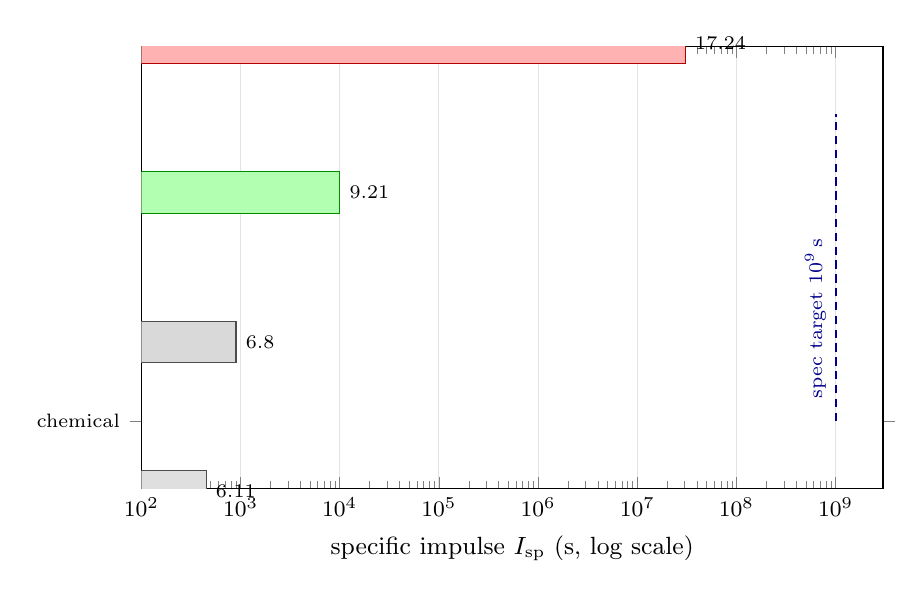
\begin{tikzpicture}
\begin{axis}[
  width=11cm, height=7.2cm,
  xbar,
  bar width=15pt,
  xmode=log,
  xmin=100, xmax=3e9,
  xlabel={specific impulse $I_{\mathrm{sp}}$ (s, log scale)},
  symbolic y coords={chemical, {fission/NTR}, {fusion/MHD (S2)}, {antimatter $c/g$ (S3)}},
  ytick=data,
  y tick label style={font=\scriptsize},
  tick label style={font=\footnotesize},
  label style={font=\small},
  nodes near coords,
  nodes near coords style={font=\scriptsize},
  xmajorgrids, grid style={gray!22},
  enlarge y limits=0.22,
]
\addplot[draw=gray!60!black,fill=gray!25] coordinates {(450,chemical)};
\addplot[draw=gray!60!black,fill=gray!30] coordinates {(900,{fission/NTR})};
\addplot[draw=green!55!black,fill=green!30] coordinates {(1e4,{fusion/MHD (S2)})};
\addplot[draw=red!70!black,fill=red!30] coordinates {(3.06e7,{antimatter $c/g$ (S3)})};
% spec target 1e9 s vertical line (above photon ceiling)
\draw[blue!55!black, thick, densely dashed] (axis cs:1e9,chemical) -- (axis cs:1e9,{antimatter $c/g$ (S3)});
\node[blue!55!black, font=\scriptsize, anchor=south, rotate=90] at (axis cs:1e9,{fission/NTR}) {spec target $10^9$\,s};
\end{axis}
\end{tikzpicture}
\end{document}
